\title{ORB.S : Open Rendering Benchmark Spec}
\author{Ray Tracing Systems}
\date{\today}

\documentclass[12pt]{article}

\usepackage[
  a4paper, mag=1000, includefoot,
  left=3cm, right=1cm, top=2cm, bottom=2cm, headsep=1cm, footskip=1cm
]{geometry}
\usepackage[T2A]{fontenc}
\usepackage[cp1251]{inputenc}
\usepackage[english]{babel} 	
\usepackage{float}
\usepackage[section]{placeins}

\usepackage{hyperref}
\hypersetup{pdfborder={0 0 0}, colorlinks=true, urlcolor=blue} % Specify a color for hyperlinks
\usepackage{todonotes} % Required for the boxes that questions appear in
\usepackage{tocloft} % Required to give customize the table of contents to display questions
\usepackage{enumitem}


\renewcommand{\baselinestretch}{1.25}
\newcommand\boldblue[1]{\textcolor{darkblue}{\textbf{#1}}}

\usepackage{xcolor} % for setting colors
\definecolor{gray}{rgb}{0.4,0.4,0.4}
\definecolor{darkblue}{rgb}{0.0,0.0,0.6}
\definecolor{cyan}{rgb}{0.0,0.5,0.5}
\definecolor{maroon}{rgb}{0.5,0,0}
\definecolor{darkgreen}{rgb}{0.0,0.5,0.0}

\usepackage{listings}
\lstdefinelanguage{XML}
{
	basicstyle=\ttfamily\footnotesize,
	morestring=[b]",
	moredelim=[s][\bfseries\color{darkblue}]{<}{\ },
	moredelim=[s][\bfseries\color{darkblue}]{</}{>},
	moredelim=[l][\bfseries\color{darkblue}]{/>},
	moredelim=[l][\bfseries\color{darkblue}]{>},
	morecomment=[s]{<?}{?>},
	morecomment=[s]{<!--}{-->},
	commentstyle=\color{darkgreen},
	stringstyle=\color{black},
	identifierstyle=\color{cyan},
	commentstyle=\color{gray}\upshape,
	keywordstyle=\color{cyan}\underbar,
	morekeywords={ver, type, brdf_type, shape, distribution}% list your attributes here
}

% set the default code style
\lstset{
	frame=leftline,                 % draw line on left of code
	tabsize=4,                      % tab space width
	showstringspaces=false,         % don't mark spaces in strings
	xleftmargin=2em,
	framexleftmargin=2em
}

% Create the command used for removed procs
\newcommand{\listreqname}{}
\newlistof{req}{def2}{\listreqname}


\newcommand{\reqirenment}[1]{%
	\refstepcounter{req}%
	\par\noindent 
	\phantomsection % Needed for hyperref compatibility with the \addcontensline command
	%\addcontentsline{def2}{figure}{#1} % Adds the question to the list of questions
	\addcontentsline{def2}{figure}
	{\protect\numberline{\thesection.\thereq}#1}\par
	\todo[inline, color=green!25]{\textbf{mat\_\thesection.\thereq:} \textbf{#1} \hyperref[ruleslist]{(core)}} % Uses the todonotes package to create a fancy box to put the question
	\vspace{1em} % White space after the question before the start of the answer
}


\newcommand{\reqirenmentg}[1]{%
	\refstepcounter{req}%
	\par\noindent 
	\phantomsection % Needed for hyperref compatibility with the \addcontensline command
	%\addcontentsline{def2}{figure}{#1} % Adds the question to the list of questions
	\addcontentsline{def2}{figure}
	{\protect\numberline{\thesection.\thereq}#1}\par
	\todo[inline, color=green!25]{\textbf{geo\_tri\_\thesection.\thereq:} \textbf{#1} \hyperref[ruleslist]{(core)}} % Uses the todonotes package to create a fancy box to put the question
	\vspace{1em} % White space after the question before the start of the answer
}


\newcommand{\reqirenmentlight}[1]{%
	\refstepcounter{req}%
	\par\noindent 
	\phantomsection % Needed for hyperref compatibility with the \addcontensline command
	%\addcontentsline{def2}{figure}{#1} % Adds the question to the list of questions
	\addcontentsline{def2}{figure}
	{\protect\numberline{\thesection.\thereq}#1}\par
	\todo[inline, color=green!25]{\textbf{lgt\_\thesection.\thereq:} \textbf{#1} \hyperref[ruleslist]{(core)}} % Uses the todonotes package to create a fancy box to put the question
	\vspace{1em} % White space after the question before the start of the answer
}


\newcommand{\reqirenmentextension}[1]{%
	\refstepcounter{req}%
	\par\noindent 
	\phantomsection % Needed for hyperref compatibility with the \addcontensline command
	%\addcontentsline{def2}{figure}{#1} % Adds the question to the list of questions
	\addcontentsline{def2}{figure}
	{\protect\numberline{\thesection.\thereq}#1}\par
	\todo[inline, color=blue!25]{\textbf{mat\_\thesection.\thereq:} \textbf{#1} \hyperref[ruleslist]{(extension)}} % Uses the todonotes package to create a fancy box to put the question
	\vspace{1em} % White space after the question before the start of the answer
}



\newcommand{\extension}[1]{%
	\refstepcounter{req}%
	\par\noindent 
	\phantomsection % Needed for hyperref compatibility with the \addcontensline command
	%\addcontentsline{def2}{figure}{#1} % Adds the question to the list of questions
	\addcontentsline{def2}{figure}
	{\protect\numberline{\thesection.\thereq}#1}\par
	\todo[inline, color=yellow!25]{\textbf{mat_ext\_\thesection.\thereq:} \textbf{#1} \hyperref[ruleslist]{(up)}} % Uses the todonotes package to create a fancy box to put the question
	\vspace{1em} % White space after the question before the start of the answer
}


\begin{document}
\maketitle

\begin{abstract}
The standard feature number definition consists of 3 parts. They are material, lights and geometry. Thus to determine a finite set of features renderer support you have to specify 3 numbers in subsequent order. For example: <<G0.1/M0.3/L0.4>> means <<0.1>> version for geometry, <<0.3>> version for materials and <<0.4>> for lights. Each number in specification definition means all <<core>> requirenments with less number are fulfilled. For example, materials ver 2.2 means 0.* and 1.* requirenemnts, 2.1 and 2.2 are implemented/fulfilled but 2.3 may be not implemented/fulfilled.

\end{abstract}

\section{List of requirenments}\label{ruleslist}

\listofreq

\section{Geometry v1.0}\label{geomfeatures}

\setcounter{section}{1}
\setcounter{req}{-1}

General requirenments: 

\boldblue{(!)REQ:} Renderer should not do any geometry preprocessing (such as normals recalculation, vertex splitting, etc.) and use provided data as it is. This is valid for all specification levels unless otherwise specified.

\reqirenmentg{primitive\_format}

The geometry should be represented as triangulated indexed meshes. Indices must be specified with uniform winding order for the whole scene - only clockwise or only counter-clockwise. Triangle vertices \textbf{must} have the following attributes specified:
\begin{itemize}
	\item positions in 3d space;
	\item normals;
	\item tangents;
	\item texture coordinates (can be set to zeroes if are not available).
\end{itemize}

For each triangle of this mesh some material is assigned --- that is, per triangle material is specified.

\reqirenmentg{single\_mesh}

At this specification level, the whole scene is defined as a single mesh or several meshes with transformed vertices in \underline{world space}. All positions of vertices must me specified \underline{in meters}. 

There are five parameters that should be specified for drawing model: (fovY, width, height, zNear, zFar). If they are not specified, renderer may use default values:

\begin{itemize}
\item fovY   -- vertical field of view in degrees, default value is 90.0.
\item width  -- image width in pixels, default value is 1024.
\item height -- image height in pixels, default value is 1024. 
\item zNear	 -- near plane in meters, default value is 0.1.
\item zFar   -- far plane in meters, default value is 100.0.
\end{itemize}

The projection matrix should be obtained from (left,right,bottom,top) in the way OpenGL standart specifies for \href{https://www.khronos.org/registry/OpenGL-Refpages/gl2.1/xhtml/glFrustum.xml}{glFrustum} according to further calculations:
\begin{eqnarray*}
aspect &=& \frac{width}{height} \\
ymax   &=& zNear * tan(fovY*\frac{\pi}{360.0}) \\
xmax   &=& ymax * aspect \\
left   &=& -xmax, right = +xmax, bottom = -ymax, top = +ymax \\
\end{eqnarray*}

Reference implementation can be found \href{https://github.com/Ray-Tracing-Systems/HydraAPI-tests/blob/dev/doc/doc_hydra_standart/cammatrices.h}{here} (perspectiveMatrix)


The camera should be specified in the following way:
\begin{itemize}
\item camera position : point in 3D.
\item camera lookAt  : point in 3D.
\item camera upVector : point in 3D, default value is (0,1,0).
\item camera distance : scalar, represent distance to focal plane.
\end{itemize}

The modelView matrix should be calculated from (position,lookAt,upVector) according to \href{https://www.khronos.org/registry/OpenGL-Refpages/gl2.1/xhtml/gluLookAt.xml}{gluLookAt} specification. Reference implementation can be found \href{https://github.com/Ray-Tracing-Systems/HydraAPI-tests/blob/dev/doc/doc_hydra_standart/cammatrices.h}{here} (lookAt).

\reqirenmentg{inst\_matrices}\label{geom3}

At this specification level, the whole scene is defined as set of instances of meshes. Each mesh instance has its own transform 4x4 matrix. Matrices can contain rotation, translation, scaling (both linear and non-linear). If the mesh was not instanced at all, it should not be drawn.

\boldblue{Test:} test\_005\_instancing.
\begin{figure}[htb]
	\centering
	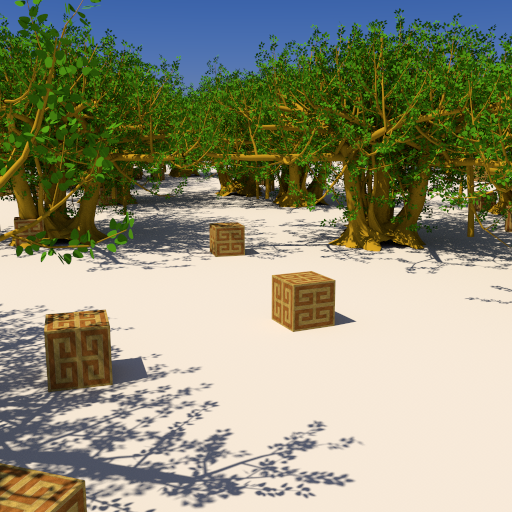
\includegraphics[width=0.4\linewidth]{../../tests_images/test_005/w_ref.png}           
	\caption{\label{fig:test_005_image}
		Example of instancing.  }   
\end{figure}

\FloatBarrier

\reqirenmentg{inst\_change\_material}

This requirement defines the ability to instantiate same objects with different materials. However, only single material for the whole mesh (and thus fo the whole instance) is allowed. Though, rasterization based traditional renderers assume to change their shaders once per instance and the ray tracing based solutions should substitute single material id for each instance. 

\boldblue{(!)Note: }In other words, each mesh has strictly 1 material, and if any of them has 2 different materials, the exporter must divide this mesh into two different meshes.

\boldblue{(!)Note: }Here we can see a unobvious thing for content exporter developers. On both previous and subsequent levels of specification for a single mesh it is allowed to have several materials. But current specification level directly forbids this: export/preparation software must split meshes to have only single material per mesh. It is important to emphasize that there is no contradiction here, because our specification is created for renderers and thus exporters must adapt to this. For render systems without full instancing support (geom: \ref{geom2}, \ref{geom3}) in general there is no difference if object was spitted to several meshes or not, as well remap list (see next spec. level) size may be equal to 1 when we go to subsequent levels. 

\reqirenmentg{inst\_remaplist\_(MaxMaterials == 4)}

This requirement defines the ability to instantiate same objects with different materials. That is, different instances of the same object can have different materials. For this, we define such a thing as <<remap list>>. The remap list is a list of pairs of material indices. In each pair, the first index defines the material to be replaced, and the second index determines the final material. For example, consider further remap lists (listing \ref{remaplist}): 

\lstset{language=XML}
\begin{lstlisting}[caption=Remap list example, label=remaplist, captionpos=b]
<remap_lists>
  <remap_list id="0" size="4" val="0 5 3 1 " />
  <remap_list id="1" size="8" val="1 0 2 0 3 0 4 0 " />
</remap_lists>
\end{lstlisting}

The remap list with id <<0>> will replace material 0 to 5 and material 3 to 1. The remap list with id <<1>> will replace all its input materials (1,2,3,4) to 0. 

So, each instance can assign an existing remap list. If this happends, for this instance on the displayed model the replacements specified in remap list should be applied (fig. \ref{fig:remaplist}).

\boldblue{Test:} test78\_material\_remap\_list1. MSE should be less than 5.0 for 512x512 LDR image.

\begin{figure}[h]\label{fig:remaplist}
	\begin{minipage}[h]{0.45\linewidth}
		\center{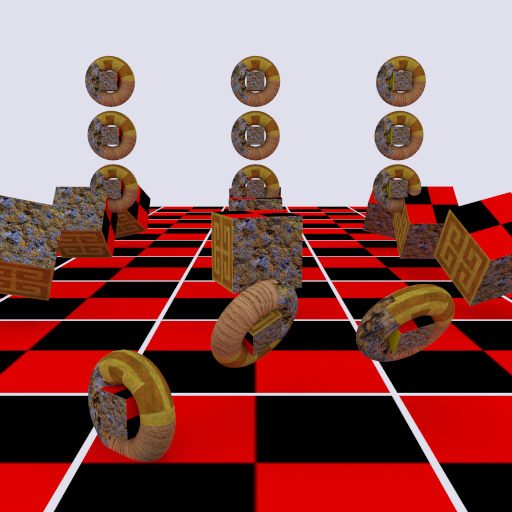
\includegraphics[width=1.0\linewidth]{../../tests_images/test_79/w_ref.png} \\ Original material mapping}
	\end{minipage}
	\begin{minipage}[h]{0.45\linewidth}
		\center{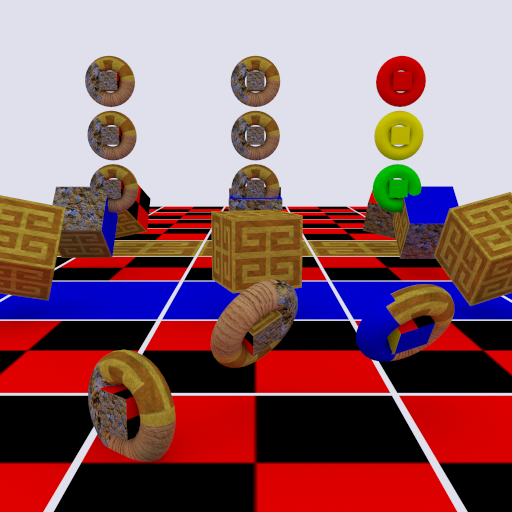
\includegraphics[width=1.0\linewidth]{../../tests_images/test_79/w_ref2.png} \\ Appliyng remap list}
	\end{minipage}
	\caption{Remap list example.}
\end{figure}

\boldblue{(!)Note: } For efficiency reasons renderers may restrict remap list size (MaxMaterials == 4). This is essential, for example for objects with opacity (leafes, grass and e.t.c). If remapped material has opacity property, during ray-triangle intersection we have to look up in the opacity texture. However, material id remapping in general case is implemented via binary search which is too expensive if performed for each triangle. In this way renderer may restrict remap list size to 4 or 8 elements (and thus 2 or 4 materials, for example) to be sure that remapping will be cheap enough. Please note that default maximum material amount in remap list is equal to 4 and thus \underline{exporter must split} single mesh to several meshes for all instances that have greater than 4 materials in their remap list.      

\FloatBarrier

\section{Materials v1.0.}\label{materialgeneral}

Image \ref{fig:brdf} and equation \ref{eq:integral} show lighting integral and related angles. These notation will be used further in the document. They assume reverse (i.e. Path Tracing) direction of light by default: 

\begin{figure}[htb]
	\centering
	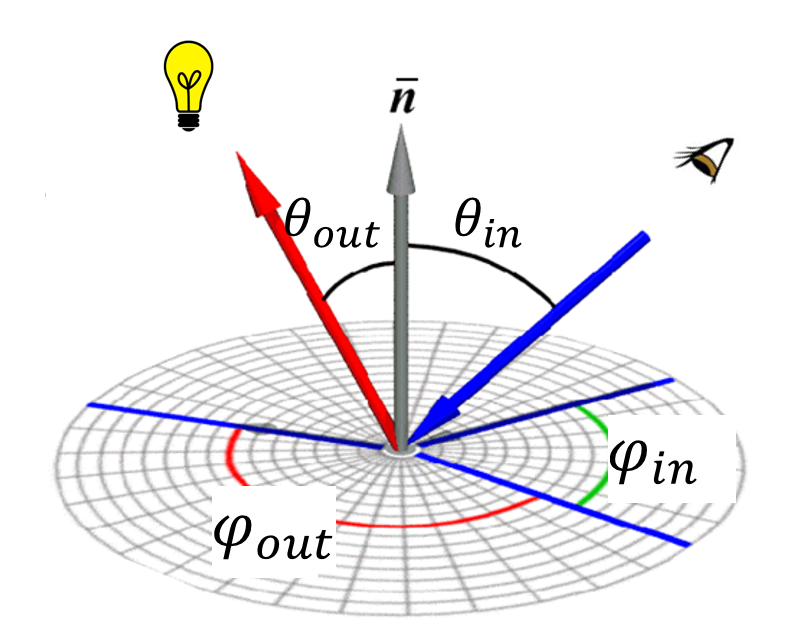
\includegraphics[width=0.3\linewidth]{images/brdf}           
	\caption{\label{fig:brdf}
		BRDF and angles.}   
\end{figure}

\begin{eqnarray}\label{eq:integral}
I(\phi_{in}, \theta_{in}) = \int\limits_{\phi_{out}}\int\limits_{\theta_{out}}  L(\phi_{out},\theta_{out})BRDF(\phi_{out},\theta_{out},\phi_{in},\theta_{in})cos(\theta_{out}) \mathrm{d}\phi_{out}  \mathrm{d}\theta_{out}
\end{eqnarray}

It should be noted that the adopted agreement of the backward propagation of light (from eye to light) does not limit anything and can be applied also for calculation of forward propagation (from light to eye).

\boldblue{(!) Implementation REQ. :} All BRDF and BTDF should be implemented without $cos(\theta_{out})$ term. For mirrors cosine shouldn't be applied, thus you should pre-divide $cos(\theta_{out})$ instead (so that the cosines cancel each other). Also note that we do not include color in BRDF/BTDF equations. The color should be multiplied with the BRDF value.

\boldblue{(!) Implementation REQ. :} Note that texture color (that comes from PNG, JPG, BMP and othe LDR formats) should be transformed to linear space with gamma transform: $ C_{linear} = C_{srgb}^{2.2} $. Unlike textures values that are \textbf{specified explicitly} in XML (or other) assummed to be \textbf{already in linear space}.

\boldblue{(!) Implementation REQ. :} Note that final color of the image should be first clamped and then transformed from HDR to LDR space with gamma correction: $ C_{srgb} = C_{linear}^{(1.0/2.2)} $. Clamping should be simple (i.e. losing color). For example color (1.5, 2.0, 10.0) should be clamped to (1,1,1) but not to (0.15, 0.2, 1.0) for example.

\boldblue{(!) Symbols:}\label{symbols} 

\begin{itemize}
\item $\omega_i = v$: in, or view vector (note that on image \ref{fig:brdf} inverse view vector (i.e. $-v$) is drawn with blue arrow);
\item $\omega_o = l$: out, or light vector;
\item $\omega_h = \frac{l+v}{2}$, half vector;
\item $n$, normal vector.
\end{itemize}


\setcounter{section}{1}
\setcounter{req}{-1}

\reqirenment{lambert}

Basic support for Lambertian reflections. The BRDF function \textbf{must} be implemented according to equation \ref{brdf_lambert}. See fig \ref{fig:test_101_image}. % and listing \ref{lambertxml} for image and XML example respectively.

\boldblue{Implementation:}
\begin{equation}\label{brdf_lambert}
BRDF_{lambert} = \frac{1}{\pi}
\end{equation}

\boldblue{Test:} 101\_diffuse\_lambert. MSE should be less than 5.0 for 512x512 LDR image.
\begin{figure}[htb]
	\centering
	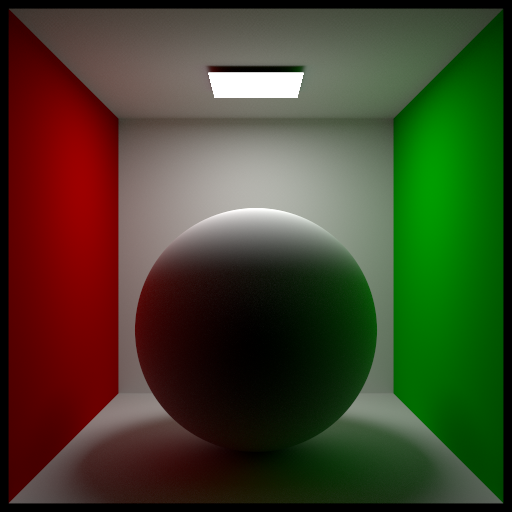
\includegraphics[width=0.25\linewidth]{../../tests_images/test_101/w_ref.png}           
	\caption{\label{fig:test_101_image}
     Example of lambertian material. The grey ball have color equal to (0.5, 0.5, 0.5).  }   
\end{figure}

\FloatBarrier

\reqirenment{emission}

Basic support for emissive material. On this level of specification emissive materials don't combined with others. Renderer may suppose mutually exclusive: (emissive or 'some other'). Please note that emissive materials have not be considered as lights (i.e. they don't have to be sampled with any explicit sampling strategy, however, of cource, they could), but they must cast GI.

\boldblue{Test:} 123\_emission. MSE should be less than 5.0 for 512x512 LDR image. 

\begin{figure}[h]
	\begin{minipage}[h]{0.26\linewidth}
		\center{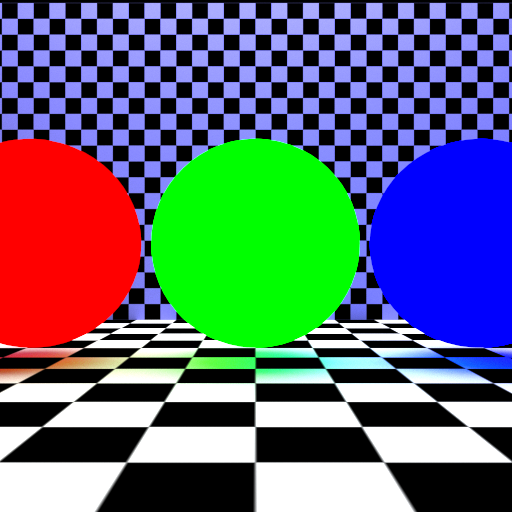
\includegraphics[width=1.0\linewidth]{../../tests_images/test_123/w_ref.png} \\ red emission}
	\end{minipage}
	\hfill
	\begin{minipage}[h]{0.26\linewidth}
		\center{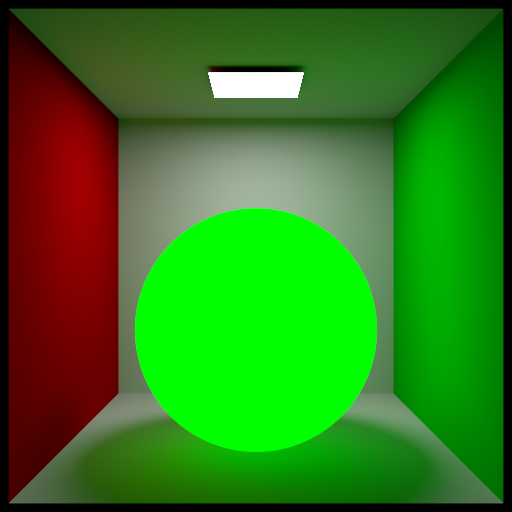
\includegraphics[width=1.0\linewidth]{../../tests_images/test_123/w_ref2.png} \\ green emission}
	\end{minipage}
    \hfill
	\begin{minipage}[h]{0.26\linewidth}
		\center{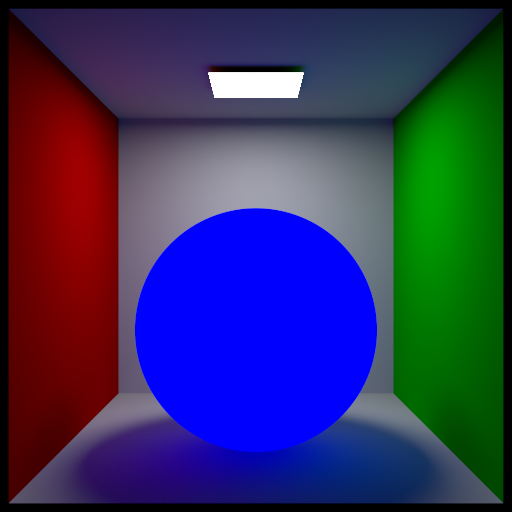
\includegraphics[width=1.0\linewidth]{../../tests_images/test_123/w_ref3.png} \\ blue emission}
	\end{minipage}
	\caption{Phong for different cosine power and color (0.5, 0.5, 0.5).}
\end{figure}

\FloatBarrier

\boldblue{(!) Implementation REQ. :} Emission color value \textbf{must} specify \textbf{brightness} value. It is easy to ckeck this requirenment. Directly visible emissive surface on rendered image (stored in linear HDR framebuffer) must have exactly same value that was set for material. For example if you set emission color to (0.5, 0.5, 0) and then check directly visible surfaces (when primary rays immediately hit surface), you shoulg get exactly same yellow color (0.5, 0.5, 0) in the rendered image (in linear space, i.e. HDR image).

\reqirenment{ggx}

The GGX isotropic BRDF implementation according to \cite{ggx} and \cite{ggxSampling}:

\begin{eqnarray*}
	A &=& \frac{1}{\omega_i \cdot n + \sqrt{ \alpha^2 + (1-\alpha^2) (\omega_i \cdot n)^2} } \\
	B &=& \frac{1}{\omega_o \cdot n + \sqrt{ \alpha^2 + (1-\alpha^2) (\omega_o \cdot n)^2} } \\
	D &=& \frac{\alpha^2}{ \pi \left( (\omega_h \cdot n)^2 . (\alpha^2 - 1) + 1 \right)^2 }  \\
	\\
	f_r(\omega_o, \omega_i, \alpha) &=& A*B*D \\
\end{eqnarray*}

Where $\alpha$ is roughness and $(\omega_o, \omega_i)$ described previously here \ref{symbols}.

GGX sampling can be efficiently implemented according to the Eric Heitz paper \cite{ggxSampling}. Additional implementation with further explanation can be found \href{https://schuttejoe.github.io/post/ggximportancesamplingpart2/}{here} \cite{ggxSampling2}.

%330_CornellBoxWithSphereCylinderTeapot

\boldblue{Test:} 330\_CornellBoxWithSphereCylinderTeapot. 
\begin{figure}[htb]
	\centering
	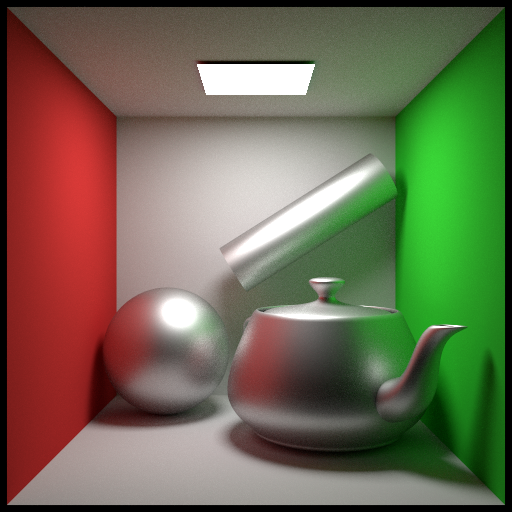
\includegraphics[width=0.30\linewidth]{../../3dsMaxTests/Reference/330_CornellBoxWithSphereCylinderTeapot.png}           
	\caption{\label{fig:CornellBoxWithSphereCylinderTeapot} testing GGX: Todo describe parameters, add make images for different roughness cases.  }   
\end{figure}

\FloatBarrier

\reqirenment{mirror}

Pure specular reflection. Note that mixing of mirror and lambertian reflections is not needed at this level of specification. Renderer may suppose mutually exclusive: (phong, mirror or lambert). 
\boldblue{Implementation:} It is assumed that you will pre-divide to $cos(\theta_{out})$ inside BRDF and later cancel this cosine in lighting integral (equation \ref{eq:integral}) instead of considering pure specular reflection as a special case during lighting integral evaluation. Though, you will probably have to consider pure specular reflection as special cases in many other places. 
\begin{equation}\label{brdf_idealmirror1}
BRDF_{mirror} = \frac{1}{cos(\theta_{out})}
\end{equation}

\boldblue{(!) Implementation Note:} You are \textbf{allowed} to clamp denominator to avoid dividing by zero: 

\begin{equation}\label{brdf_idealmirror2}
BRDF_{mirror} = \frac{1}{\max(cos(\theta_{out}), 10^{-6})}
\end{equation}

\boldblue{Test:} test\_174\_mirror\_orbspec\_mat03. 
\begin{figure}[htb]
	\centering
	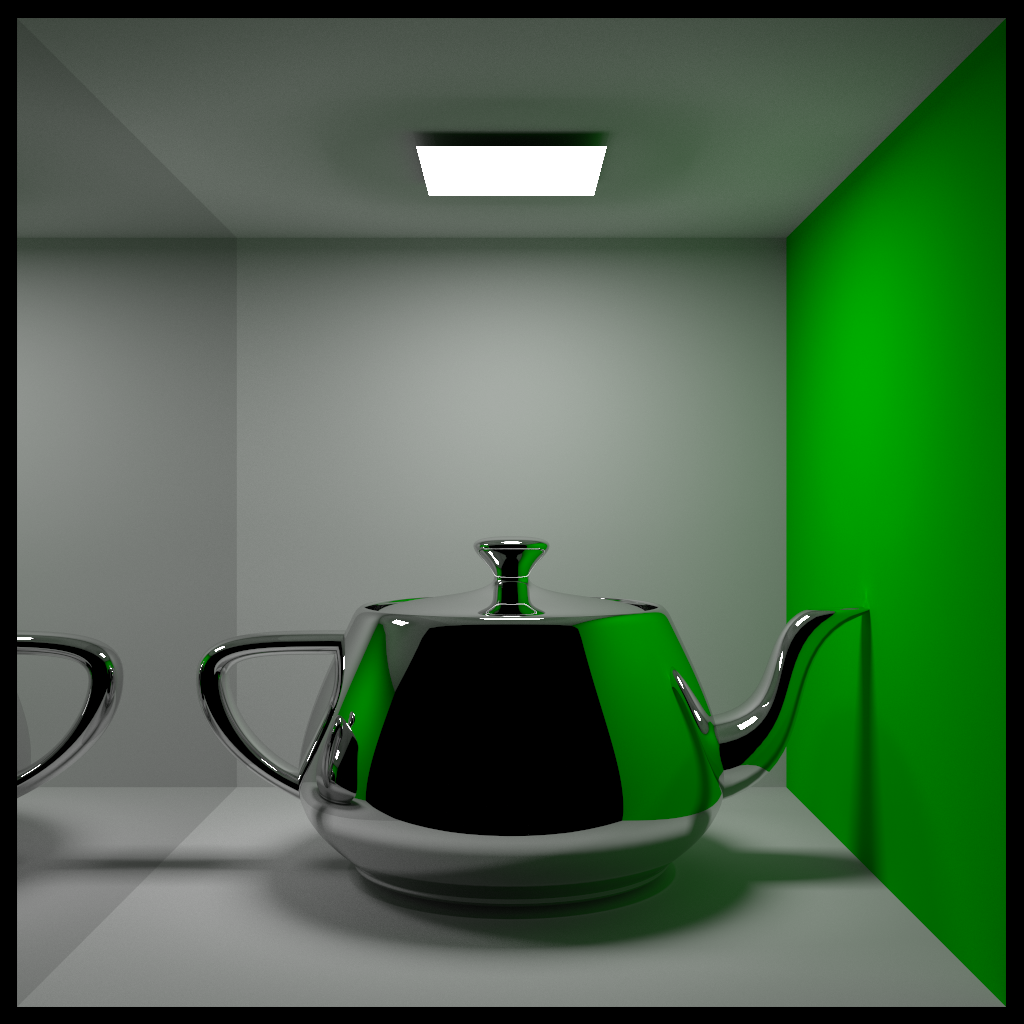
\includegraphics[width=0.25\linewidth]{../../tests_images/test_174/w_ref.png}           
	\caption{\label{fig:test_174_image}
		Example of mirror material with color equal to (0.75, 0.75, 0.75).  }   
\end{figure}

\reqirenment{lambert\_texture\_color}\label{req:diffusetexture}

Adding LDR textures for Lambertian materials. When reading from LDR texture, gamma transform \textbf{should} be applied. The resulting color must be the product of texture color and material color. Texture matrices support is not needed on this level of specification.

\boldblue{Test:} test\_103\_diffuse\_texture. MSE should be less than 5.0 for 512x512 LDR image. 
\begin{figure}[htb]
	\centering
	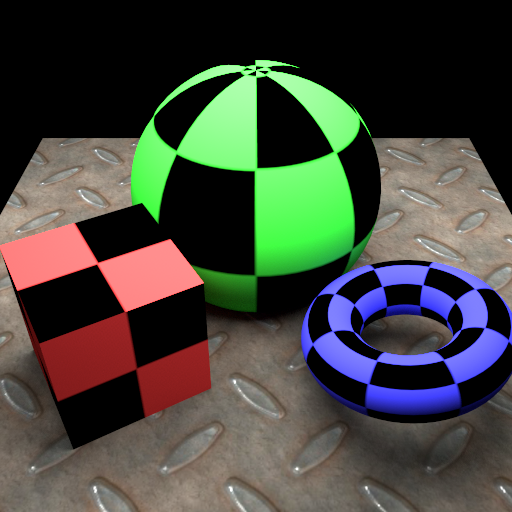
\includegraphics[width=0.25\linewidth]{../../tests_images/test_103/w_ref.png}           
	\caption{\label{fig:test_103_image}
		Example of lambertian material with textures.  }   
\end{figure}

\FloatBarrier

\reqirenment{reflect\_texture\_color}

Adding LDR textures for reflection color for both ggx and mirrors. When reading from LDR texture, gamma transform \textbf{should} be applied. The resulting color must be the product of texture color and material color. Texture matrices support is not needed on this level of specification.

\boldblue{Test:} test\_108\_reflect\_texture. MSE should be less than 5.0 for 512x512 LDR image. 
\begin{figure}[htb]
	\centering
	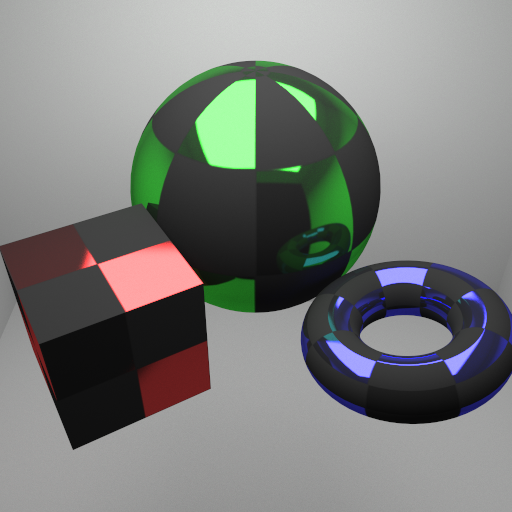
\includegraphics[width=0.25\linewidth]{../../tests_images/test_108/w_ref.png}           
	\caption{\label{fig:test_108_image}
		Example of phong material with textures.  }   
\end{figure}

\FloatBarrier

\boldblue{(!) Implementation REQ. :} Texture fetch (samplers) must support both <<wrap>> and <<clamp>> addressing modes separately for $u$ and $v$ texture coordinates. Please see req. \ref{req:diffusetexture} for detailed description.

\reqirenment{emission\_texture\_color\_ldr}

Adding LDR textures to emission color. When reading from LDR texture, gamma transform \textbf{should} be applied. The resulting color must be the product of texture color and material color. Texture matrices support is not needed on this level of specification.

\boldblue{Test:} test\_124\_emission\_texture. MSE should be less than 5.0 for 512x512 LDR image. 
\begin{figure}[htb]
	\centering
	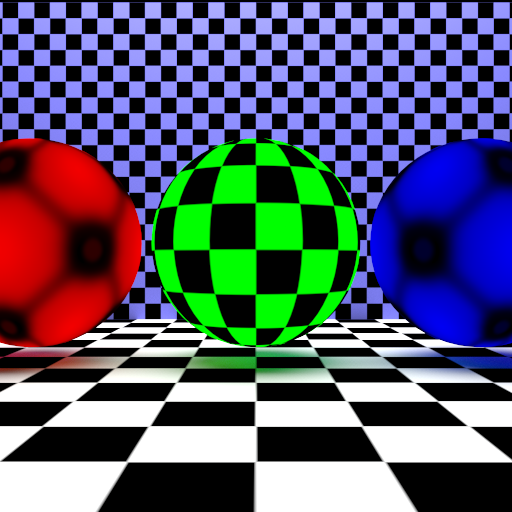
\includegraphics[width=0.25\linewidth]{../../tests_images/test_124/w_ref.png}           
	\caption{\label{fig:test_124_image}
		Emissive textures.  }   
\end{figure}

\FloatBarrier

\reqirenment{ggx\_texture\_glosiness}

Adding textures for reflection $glosiness = 1-roughness$ in ggx model. Colored textures should use $max(color.r, color.g, color.b)$ to get glosiness value from textures.

\boldblue{Note:} On this specification level ggx with glosiness equal to 1 \textbf{must} become mirror material.

\reqirenment{texture\_wrap\_and\_clamp}

Texture fetch (samplers) must support both <<wrap>> and <<clamp>> addressing modes separately for $u$ and $v$ texture coordinates. If the mode is not specified, the default mode is wrap.  Lack of support for the <<clamp>> mode in test (req.\ref{req:diffusetexture}) will lead to incorrect visualization of the edges of the cube due to interpolation between red and black colors, which should be absent with the <<clamp>> mode. Texture sampler parameters must be enabled for further material parameters: diffuse, reflection, emission, glosiness.

\reqirenment{texture\_matrices}

The sampler object must support the storage and use of texture matrices. Texture matrices are aplied to texture coordinates before actual texture fetch is performed. Initially, the matrices should be 4x4, but since in most cases the texture coordinates are two-dimensional, at this level of the specification, the render can save only the first 2 rows of the matrix.

\reqirenment{mix\_ggx\_lambert\_extrusion\_maxcolor}

Mixing ggx and lambert. The ggx reflection have a higher priority and \textbf{must} extrude Lambertian reflection if summ of reflection coefficients are greater than 1.

Colored textures gain $max(color.r, color.g, color.b)$ for mix coefficient.

\reqirenment{mix\_ggx\_lambert\_extrusion\_avgcolor}

Mixing ggx and lambert. The ggx reflection have a higher priority and \textbf{must} extrude Lambertian reflection if summ of reflection coefficients are greater than 1. The Corona and Mental Ray renderers use this extrusion type by default.

Colored textures gain $avg(color.r, color.g, color.b)$ for mix coefficient.


\reqirenmentextension{mix\_ggx\_lambert\_extrusion\_percomponent}

Mixing ggx and lambert separately for each color component.  The ggx reflection have a higher priority and \textbf{must} extrude lambertian reflection \textit{separately for each color component} if summ of reflection coefficients are greater than 1. The VRay renderer use this extrusion type by default.

\reqirenmentextension{mix\_ggx\_lambert\_extrusion\_sumcolor}

Mixing ggx and lambert without priority. If summ of reflection coefficients is greater than 1, both of them \textbf{should} be scaled linearly to get sum equal to 1.0 \textit{separately for each color component}.

Note that all mixtures could be (and in general recommended to be) implemented via blend by mask (see blend\_mask). However, on this level of specification you don't have to implement blend for BRDFs.



\addtocounter{section}{2}


\section{Light v1.0}\label{lightfeatures}

\setcounter{section}{1}
\setcounter{req}{-1}

\reqirenmentlight{area\_light}

\begin{thebibliography}{1}
\small{    
		
\bibitem{fixedpaper} Eric P. Lafortune and Yves D. Willems. \textit{Using the Modified Phong Reflectance Model for Physically Based Rendering}. 1994. 
		
		
\bibitem{ggx} Bruce Walter, Stephen R. Marschner, Hongsong Li, and Kenneth E. Torrance.  \textit{Microfacet models for refraction through rough surfaces.} In Proceedings of the 18th Eurographics conference on Rendering Techniques (EGSR�07). 2007. Eurographics Association, Goslar, DEU, 195�206.		
		
\bibitem{ggxSampling} Eric Heitz. \textit{A Simpler and Exact Sampling Routine for the GGX Distribution of Visible Normals.} [Research Report] Unity Technologies. 2017. hal-01509746		

\bibitem{ggxSampling2} Joe Schutte. \textit{Importance Sampling techniques for GGX with Smith Masking-Shadowing: Part 2}. March 7, 2018. Github pages, accessed 22.05.2020. 		
		
}
\end{thebibliography}


\end{document}




